\documentclass[%
 twocolumn,
 superscriptaddress,
%groupedaddress,
%unsortedaddress,
%runinaddress,
%frontmatterverbose,
%showpacs,
 preprintnumbers,
 nofootinbib,
%nobibnotes,
%bibnotes,
 amsmath,amssymb,
 aps,
 prl,
%pra,
%prb,
%rmp,
%prstab,
%prstper,
%floatfix,
]{revtex4-2}
\usepackage{psfrag,slashed,cancel,array,graphicx,hyperref}
\usepackage{subfigure}
%\usepackage[justification=justified]{subcaption}
% \usepackage[labelfont=bf,labelsep=quad,justification=justified]{caption}
\usepackage[utf8]{inputenc}
\usepackage{mathtools}
\usepackage{mathrsfs}
\usepackage{multirow}
\usepackage{braket}
\usepackage{booktabs} %nice tables
\usepackage[normalem]{ulem}
\hypersetup{pdftitle={},pdfcreator={},linkcolor=[rgb]{0.15,0.35,0.75},colorlinks=true,citecolor=[rgb]{0.675,0,0.2},urlcolor=[rgb]{0.15,0.35,0.65}}

% The Letter of the single-paper layout (REVTeX 4.2, PRL). Every number quoted in the text and in Table I
% is a macro defined in numbers.tex, and the two tables of the End Matter are in tables/; all are written
% by make_tables.py from the result files, through the shared generators
% (../_build). Fig. 1 is a TikZ-Feynman diagram (figures/dps_diagram_tikz.tex), compiled by make_figure.py
% from figures/dps_diagram.tex. `make` rebuilds everything and asserts the PRL length limits with
% count_words.py.
% generated by make_tables.py from the result files; do not edit
\newcommand{\devLeadMax}{\ensuremath{7\times10^{-12}}}
\newcommand{\vanishMax}{\ensuremath{3\times10^{-13}}}
\newcommand{\shiftMax}{\ensuremath{6\times10^{-10}}}
\newcommand{\plainDevMax}{\ensuremath{10^{-6}}}
\newcommand{\colourTableBeta}{\ensuremath{\frac12}}
\newcommand{\imagMax}{\ensuremath{7\times10^{-12}}}
\newcommand{\extraPowerMax}{\ensuremath{3\times10^{-11}}}
\newcommand{\devOneLoopMax}{\ensuremath{3\times10^{-17}}}
\newcommand{\devKMax}{\ensuremath{2\times10^{-19}}}
\newcommand{\treeMax}{\ensuremath{3\times10^{-35}}}
\newcommand{\oneLoopShiftMax}{\ensuremath{3\times10^{-15}}}
\newcommand{\absentMax}{\ensuremath{8\times10^{-12}}}
\newcommand{\scaleSpread}{\ensuremath{2\times10^{-12}}}
\newcommand{\scaleSlopeDev}{\ensuremath{8\times10^{-12}}}
\newcommand{\storedMaxDiff}{\ensuremath{4\times10^{-18}}}
\newcommand{\precisionCtrl}{\ensuremath{8\times10^{-35}}}
\newcommand{\ctrlDelta}{\ensuremath{10^{-10}}}
\newcommand{\ctrlBeta}{\ensuremath{\frac12}}
\newcommand{\ctrlExtraDigits}{\ensuremath{15}}
\newcommand{\kOneSlopeSpread}{\ensuremath{7\times10^{-6}}}
\newcommand{\scanBetas}{\ensuremath{\frac14,\frac12,\frac23}}
\newcommand{\scanDeltaFirst}{\ensuremath{10^{-4}}}
\newcommand{\scanDeltaLast}{\ensuremath{10^{-11}}}
\newcommand{\digitsBase}{\ensuremath{30}}
\newcommand{\digitsPerDecade}{\ensuremath{3}}
\newcommand{\pTsqMin}{\ensuremath{2.5\times10^{-12}}}
\newcommand{\pTsqMax}{\ensuremath{6.7\times10^{-5}}}
\newcommand{\pOneKoneDev}{\ensuremath{2\times10^{-34}}}
\newcommand{\pOneAALogDev}{\ensuremath{3\times10^{-15}}}
\newcommand{\pOneHHLogDev}{\ensuremath{3\times10^{-15}}}
\newcommand{\boseDevMone}{\ensuremath{4\times10^{-24}}}
\newcommand{\boseDevMtwo}{\ensuremath{6\times10^{-32}}}
\newcommand{\hhLiValueDev}{\ensuremath{9\times10^{-44}}}
\newcommand{\zzBetas}{\ensuremath{\frac14,\frac12,\frac23}}
\newcommand{\zzDeltaFirst}{\ensuremath{10^{-4}}}
\newcommand{\zzDeltaLast}{\ensuremath{10^{-12}}}
\newcommand{\zzDigitsBase}{\ensuremath{30}}
\newcommand{\zzDigitsPerDecade}{\ensuremath{5}}
\newcommand{\zzCtrlDelta}{\ensuremath{10^{-10}}}
\newcommand{\zzCtrlBeta}{\ensuremath{\frac12}}
\newcommand{\zzPrecisionCtrl}{\ensuremath{4\times10^{-37}}}
\newcommand{\zzOneLoopDev}{\ensuremath{5\times10^{-18}}}
\newcommand{\zzRouteBCAbeta}{\ensuremath{\frac12}}
\newcommand{\zzVanishMax}{\ensuremath{2\times10^{-18}}}
\newcommand{\zzLogDevMax}{\ensuremath{2\times10^{-11}}}
\newcommand{\zzKDevMax}{\ensuremath{4\times10^{-10}}}
\newcommand{\zzDevMax}{\ensuremath{4\times10^{-10}}}
\newcommand{\zzShiftMax}{\ensuremath{3\times10^{-8}}}
\newcommand{\zzKcubicMax}{\ensuremath{9\times10^{-13}}}
\newcommand{\zzNoLogMax}{\ensuremath{6\times10^{-10}}}
\newcommand{\zzLowerModelDev}{\ensuremath{2\times10^{-7}}}
\newcommand{\zzTableBeta}{\ensuremath{\frac12}}
\newcommand{\zzTensorDev}{\ensuremath{4\times10^{-40}}}
\newcommand{\zzBenchOneLoop}{\ensuremath{7\times10^{-57}}}
\newcommand{\zzBenchCF}{\ensuremath{3\times10^{-56}}}
\newcommand{\zzBenchCA}{\ensuremath{2\times10^{-56}}}
\newcommand{\zzForwardCA}{\ensuremath{4\times10^{-21}}}
\newcommand{\zzForwardCF}{\ensuremath{3\times10^{-21}}}
\newcommand{\zzForwardCFBeta}{\ensuremath{\frac12}}
\newcommand{\zzForwardCFDelta}{\ensuremath{10^{-4}}}
\newcommand{\zzCxxBenchOneLoop}{\ensuremath{2\times10^{-30}}}
\newcommand{\zzCxxBenchTwo}{\ensuremath{2\times10^{-28}}}
\newcommand{\zzCxxFwdOneLoop}{\ensuremath{3\times10^{-19}}}
\newcommand{\zzCxxFwdCF}{\ensuremath{10^{-16}}}
\newcommand{\zzCxxFwdCA}{\ensuremath{4\times10^{-16}}}
\newcommand{\zzCxxFwdBeta}{\ensuremath{\frac12}}
\newcommand{\zzCxxFwdDelta}{\ensuremath{10^{-4}}}
\newcommand{\zzLiValueDev}{\ensuremath{3\times10^{-25}}}
\newcommand{\zzpTsqMin}{\ensuremath{2.5\times10^{-13}}}
\newcommand{\zzpTsqMax}{\ensuremath{6.7\times10^{-5}}}
\newcommand{\windowBeta}{\ensuremath{\frac12}}
\newcommand{\dpsOnset}{\ensuremath{10^{-4}}}
\newcommand{\aaRealLogDev}{\ensuremath{10^{-28}}}
\newcommand{\aaApproachBelow}{\ensuremath{10^{-6}}}
\newcommand{\nFourCuspFour}{\ensuremath{- 4 \zeta_{3}^{2} - \frac{219 \zeta_{6}}{2}}}
\newcommand{\nFourConstants}{\ensuremath{\kappa_1&=\zeta_{2},\\
\kappa_2&=\frac{\zeta_{4}}{2}, &\qquad B^{(2)}&=3 \zeta_{3},\\
\kappa_3&=- \frac{14 \zeta_{3}^{2}}{3} - \frac{13 \zeta_{6}}{24}, &\qquad B^{(3)}&=- 2 \zeta_{2} \zeta_{3} - 10 \zeta_{5},\\
\kappa_4&=- \frac{13 \zeta_{2} \zeta_{3}^{2}}{6} + \frac{65 \zeta_{3} \zeta_{5}}{2} + \frac{257 \zeta_{8}}{36}, &\qquad B^{(4)}&=5 \zeta_{2} \zeta_{5} + \frac{21 \zeta_{3} \zeta_{4}}{2} + \frac{175 \zeta_{7}}{4}.}}
\newcommand{\kernX}{\ensuremath{0.75}}
\newcommand{\kernLamMax}{\ensuremath{10^{-2}}}
\newcommand{\kernLamMin}{\ensuremath{10^{-3}}}
\newcommand{\kernSlopeDev}{\ensuremath{4\times10^{-3}}}
\newcommand{\kernRealDev}{\ensuremath{4\times10^{-4}}}
\newcommand{\kernUsDev}{\ensuremath{7\times10^{-5}}}
\newcommand{\kernUsLam}{\ensuremath{10^{-4}}}
\newcommand{\rzFitHH}{\ensuremath{5.4\times10^{-10}}}
\newcommand{\rzFitZZ}{\ensuremath{1.6\times10^{-9}}}
\newcommand{\rzBlindHH}{\ensuremath{1.7\times10^{-9}}}
\newcommand{\rzBlindZZ}{\ensuremath{4.3\times10^{-9}}}
\newcommand{\rzBlindHHunc}{\ensuremath{1.3\times10^{-7}}}
\newcommand{\rzBlindZZunc}{\ensuremath{2.7\times10^{-7}}}
\newcommand{\rzRegQ}{\ensuremath{8.4\times10^{-8}}}
\newcommand{\rzRegG}{\ensuremath{5.9\times10^{-8}}}
\newcommand{\rzEta}{\ensuremath{9.3\times10^{-14}}}
\newcommand{\rzPole}{\ensuremath{2.1\times10^{-9}}}
\newcommand{\rzSpread}{\ensuremath{1.5\times10^{-7}}}
\newcommand{\rzJspread}{\ensuremath{1.0\times10^{-7}}}
\newcommand{\rzImag}{\ensuremath{2.6\times10^{-10}}}
\newcommand{\rzQuad}{\ensuremath{5.4\times10^{-8}}}
\newcommand{\rzAlias}{\ensuremath{3.9\times10^{-6}}}
\newcommand{\rzQuadDev}{\ensuremath{5.7\times10^{-9}}}
\newcommand{\uvLeadOne}{\ensuremath{7.8\times10^{-12}}}
\newcommand{\uvPtwoOne}{\ensuremath{4.1\times10^{-8}}}
\newcommand{\uvWindowOne}{\ensuremath{4.5\times10^{-10}}}
\newcommand{\uvMatchingOne}{\ensuremath{2.0\times10^{-10}}}
\newcommand{\uvCOneOne}{\ensuremath{3.3\times10^{-18}}}
\newcommand{\uvLeadTwo}{\ensuremath{7.3\times10^{-12}}}
\newcommand{\uvPtwoTwo}{\ensuremath{2.2\times10^{-8}}}
\newcommand{\uvWindowTwo}{\ensuremath{4.6\times10^{-10}}}
\newcommand{\uvMatchingTwo}{\ensuremath{1.8\times10^{-10}}}
\newcommand{\uvCOneTwo}{\ensuremath{6.4\times10^{-18}}}
\newcommand{\rzBoundHH}{\ensuremath{4.1\times10^{-8}}}
\newcommand{\rzBoundZZ}{\ensuremath{1.0\times10^{-7}}}
\newcommand{\rzRatioHH}{\ensuremath{0.02}}
\newcommand{\rzRatioZZ}{\ensuremath{0.02}}
\newcommand{\rzIdentRes}{\ensuremath{4.9\times10^{-8}}}
\newcommand{\rzIdentC}{\ensuremath{3.2\times10^{-9}}}
\newcommand{\rzZZspread}{\ensuremath{4.8\times10^{-11}}}
\newcommand{\kappaOneReg}{\ensuremath{2.1\times10^{-7}}}
\newcommand{\nFourFDH}{\ensuremath{2.2\times10^{-13}}}
\newcommand{\rzNfourPole}{\ensuremath{3.6\times10^{-9}}}
\newcommand{\rzNfourEta}{\ensuremath{4.8\times10^{-13}}}
\newcommand{\rzNfourImag}{\ensuremath{1.3\times10^{-9}}}
\newcommand{\rzNfourClosed}{\ensuremath{4.1\times10^{-7}}}
\newcommand{\rzNfourSpread}{\ensuremath{4.3\times10^{-7}}}
\newcommand{\rzNfourQuad}{\ensuremath{5.5\times10^{-8}}}
\newcommand{\rzNfourAlias}{\ensuremath{4.1\times10^{-7}}}
\newcommand{\glauberGraph}{\ensuremath{1.3\times10^{-4}}}
\newcommand{\glauberImag}{\ensuremath{3.4\times10^{-9}}}
\newcommand{\glauberImagRatio}{\ensuremath{0.02}}
\newcommand{\glauberPair}{\ensuremath{3.1\times10^{-11}}}
\newcommand{\glauberSum}{\ensuremath{2.5\times10^{-6}}}
\newcommand{\glauberRatio}{\ensuremath{5\times10^{5}}}
\newcommand{\glauberG}{\ensuremath{5.6\times10^{-11}}}
\newcommand{\glauberCancel}{\ensuremath{1.1\times10^{-6}}}
\newcommand{\csDgammaNFour}{\ensuremath{-\tfrac{\zeta_{3}}{2}a^2+\big(\tfrac{5 \zeta_{2} \zeta_{3}}{3} + 2 \zeta_{5}\big)a^3-\big(8 \zeta_{2} \zeta_{5} + 12 \zeta_{3} \zeta_{4} + \tfrac{75 \zeta_{7}}{8}\big)a^4}}
\newcommand{\csGammaRapNFour}{\ensuremath{\tfrac{7 \zeta_{3}}{2}a^2-\big(\tfrac{11 \zeta_{2} \zeta_{3}}{3} + 12 \zeta_{5}\big)a^3+\big(13 \zeta_{2} \zeta_{5} + \tfrac{45 \zeta_{3} \zeta_{4}}{2} + \tfrac{425 \zeta_{7}}{8}\big)a^4}}
\newcommand{\csDtwo}{\ensuremath{\big(\frac{404}{27}-14\zeta_3\big)C_A-\frac{112}{27}T_Fn_f}}
\newcommand{\rzFitAA}{\ensuremath{6.4\times10^{-10}}}
\newcommand{\rzAAnuTwo}{\ensuremath{1.0\times10^{-10}}}
\newcommand{\rzAAnuZero}{\ensuremath{6.4\times10^{-10}}}
\newcommand{\rzAAimag}{\ensuremath{6.3\times10^{-10}}}
\newcommand{\rzAAvanish}{\ensuremath{6.3\times10^{-12}}}
\newcommand{\rzAAlead}{\ensuremath{8.2\times10^{-12}}}
\newcommand{\rzAALogShift}{\ensuremath{7.3\times10^{-10}}}
\newcommand{\rzAAleadVanish}{\ensuremath{2.4\times10^{-13}}}
\newcommand{\rzAAoneLoop}{\ensuremath{1.2\times10^{-14}}}
\newcommand{\rzAAoneLoopNf}{\ensuremath{7.6\times10^{-16}}}
\newcommand{\rzAActrl}{\ensuremath{1.5\times10^{-74}}}
\newcommand{\rzBoundAA}{\ensuremath{4.9\times10^{-8}}}
\newcommand{\aaDeltaFirst}{\ensuremath{10^{-4}}}
\newcommand{\aaDeltaLast}{\ensuremath{10^{-11}}}
\newcommand{\rzAAparity}{\ensuremath{2.1\times10^{-10}}}
\newcommand{\rzAAoverlap}{\ensuremath{2.0\times10^{-9}}}
\newcommand{\rzBlindAA}{\ensuremath{2.0\times10^{-9}}}
\newcommand{\rzBlindAAunc}{\ensuremath{1.5\times10^{-7}}}
\newcommand{\aaBlindBetas}{\ensuremath{\frac{1}{10},\frac45}}
\newcommand{\hhLiGuard}{15}
\newcommand{\velocityCount}{three}
\newcommand{\lValueCount}{three}
\newcommand{\kOneApproachDecades}{five}
\newcommand{\storedCount}{28}
\newcommand{\kOneApproachDigits}{five}
\newcommand{\zzVelocityCount}{three}
\newcommand{\zzDeltaCount}{nine}
\newcommand{\zzCtrlExtraDigits}{15}
\newcommand{\zzLiCalls}{401}
\newcommand{\zzLiSwapped}{159}
\newcommand{\zzBenchOneLoopCount}{20}
\newcommand{\zzForwardCFDigits}{40}
\newcommand{\zzForwardCFCount}{36}
\newcommand{\zzBenchCFList}{$A_{1}$, $A_{3}$, $A_{10}$ and $A_{17}$}
\newcommand{\zzBenchCFListX}{$A_{2}$}
\newcommand{\zzLiValuePoints}{the benchmark point and at $\delta=10^{-12}$, the smallest value of the scan, for all three velocities}
\newcommand{\zzPzeroStatements}{1613}
\newcommand{\zzLiScanArgs}{7163}
\newcommand{\zzLiScanDigits}{three}
\newcommand{\zzFwdDigits}{five}
\newcommand{\zzFwdDecades}{six}
\newcommand{\aaApproachDigits}{five}
\newcommand{\aaApproachDecades}{five}
\newcommand{\nFourChecked}{25}
\newcommand{\nFourPass}{16}
\newcommand{\nFourFixed}{eight}
\newcommand{\nFourLoops}{five}
\newcommand{\nFourNmhvChecked}{15}
\newcommand{\nFourNmhvPass}{15}
\newcommand{\nFourNmhvFive}{&\tfrac{1}{384}\,\ln^8|\delta_*|\notag\\
&-\tfrac{1}{48}\,\ln^7|\delta_*|\notag\\
&+\big(\tfrac{\zeta_{2}}{24}+\tfrac{7}{48}\big)\,\ln^6|\delta_*|\notag\\
&+\big(\tfrac{5 \zeta_{3}}{24}-\tfrac{\zeta_{2}}{4}-\tfrac{7}{8}\big)\,\ln^5|\delta_*|\notag\\
&+\big(\tfrac{9 \zeta_{4}}{8}-\tfrac{25 \zeta_{3}}{24}+\tfrac{5 \zeta_{2}}{4}+\tfrac{35}{8}\big)\,\ln^4|\delta_*|\notag\\
&+\big(2 \zeta_{5}+\tfrac{7 \zeta_{2} \zeta_{3}}{3}-\tfrac{9 \zeta_{4}}{2}+\tfrac{25 \zeta_{3}}{6}-5 \zeta_{2}-\tfrac{35}{2}\big)\,\ln^3|\delta_*|\notag\\
&+\big(\tfrac{115 \zeta_{6}}{12}+4 \zeta_{3}^{2}-6 \zeta_{5}-7 \zeta_{2} \zeta_{3}+\tfrac{27 \zeta_{4}}{2}-\tfrac{25 \zeta_{3}}{2}+15 \zeta_{2}+\tfrac{105}{2}\big)\,\ln^2|\delta_*|\notag\\
&+\big(-\tfrac{55 \zeta_{7}}{4}+11 \zeta_{3} \zeta_{4}+17 \zeta_{2} \zeta_{5}-\tfrac{115 \zeta_{6}}{6}-8 \zeta_{3}^{2}+12 \zeta_{5}+14 \zeta_{2} \zeta_{3}-27 \zeta_{4}\notag\\
&\quad +25 \zeta_{3}-30 \zeta_{2}-105\big)\,\ln|\delta_*|\notag\\
&+\big(\tfrac{257 \zeta_{8}}{36}+\tfrac{45 \zeta_{3} \zeta_{5}}{2}+\tfrac{\zeta_{2} \zeta_{3}^{2}}{2}-11 \zeta_{3} \zeta_{4}-17 \zeta_{2} \zeta_{5}+\tfrac{55 \zeta_{7}}{4}+\tfrac{115 \zeta_{6}}{6}+8 \zeta_{3}^{2}\notag\\
&\quad -12 \zeta_{5}-14 \zeta_{2} \zeta_{3}+27 \zeta_{4}-25 \zeta_{3}+30 \zeta_{2}+105\big)}
\newcommand{\kernSlopePoints}{five}
\newcommand{\rzXvalues}{$x=0.1$, $0.3$ and $0.5$}
\newcommand{\rzScanX}{$x=\frac58$, $\frac34$ and $\frac56$}
\newcommand{\nFourRegPairs}{fifteen}
\newcommand{\nFourRegFracs}{$x=\frac{1}{10}$, $\frac{3}{10}$, $\frac12$, $\frac{7}{10}$ and $\frac{9}{10}$}
\newcommand{\glauberConfigs}{eighteen}
\newcommand{\glauberProcs}{$gg\to HH$, $gg\to AA$ and $gg\to ZZ$}
\newcommand{\glauberValues}{104}
\newcommand{\nFourNmhvFiveCount}{nine}
\newcommand{\nFourNmhvLower}{16}
\newcommand{\usTwoGluonGraphs}{41}
\newcommand{\usTwoGluonLeading}{twelve}
\newcommand{\usDimLow}{six}
\newcommand{\usDimHigh}{seven}
\newcommand{\csLoops}{four}
\newcommand{\csColourFactors}{42}
\newcommand{\aaPointCount}{80}
\newcommand{\aaLossFour}{46}
\newcommand{\aaLossEight}{58}


\newcommand{\LL}{\mathcal L}
\newcommand{\G}{\mathcal G}
\newcommand{\M}{\mathcal M}
\newcommand{\kk}{\boldsymbol k}
\newcommand{\qq}{\boldsymbol q}
\newcommand{\bb}{\boldsymbol b}
\newcommand{\DD}{\Delta_C}
\newcommand{\DG}{D_\gamma}
\newcommand{\Kt}{\widetilde{\mathcal K}}

\begin{document}

\title{Double parton scattering singularities in two-loop gluon-fusion amplitudes}

\author{Arunima Bhattacharya\,\href{https://orcid.org/0000-0003-4409-0901}{
\includegraphics[scale=0.05]{orcidid.pdf}}}
\affiliation{Theory Division, IFIC, University of Valencia-CSIC,\\
E-46980 Paterna, Valencia, Spain}
%
%\author{Arunima Bhattacharya}
\email{arunimab@ific.uv.es}
%\affiliation{Theory Division, IFIC, University of Valencia-CSIC, E-46980 Paterna, Valencia, Spain}

\begin{abstract}
Gluon fusion to two massive colour singlets can develop a double parton scattering (DPS) singularity as $p_T\to0$, where each gluon splits and its daughters fuse pairwise. We determine its two-loop logarithms from the renormalisation group of a common kernel and derive the finite matching functions analytically, for gluon and quark splittings. A single colour factor, of opposite sign for the two splittings, controls the cubic logarithm and a Glauber phase. Complete two-loop $gg\to HH$, $AA$ and $ZZ$ amplitudes confirm the predictions, which extend to pairs such as $\gamma^*\gamma^*$ and $W^+W^-$.
\end{abstract}

\maketitle

\textit{Introduction:} In gluon-fusion amplitudes with massless internal
partons, production of two massive colour singlets can develop a double
parton scattering (DPS) singularity as the transverse momentum $p_T$
vanishes~\cite{Gaunt:2011xd,Diehl:2011yj}: each incoming gluon splits
into two nearly on-shell partons, which fuse pairwise in two hard
subprocesses [Fig.~\ref{fig:dps}]. This occurs in a loop amplitude and has the kinematic structure of double parton scattering. Such amplitudes arise, for example, in calculations of Higgs and electroweak boson pairs at higher orders in QCD~\cite{Glover:1988rg,Banerjee:2018lfq,vonManteuffel:2015msa}.
At two loops, the colour factor $\DD$ controls
the cubic DPS logarithm, whose coefficient
changes sign between gluon and quark splittings.
The same colour factor determines the phase
in Eq.~(\ref{eq:gammaK}), tested against
complete amplitudes below.
In cross sections, the squared one-loop amplitude overlaps with
double parton scattering~\cite{Gaunt:2011xd,Manohar:2012pe,Gaunt:2012dd};
its DPS limit is subtracted to avoid double
counting~\cite{Diehl:2017kgu,BDFS2011,BDFS2012,BDFS2014}. Our two-loop terms give this
limit for the virtual corrections.
At one loop, the DPS singularity is at most logarithmic and is described
by two splitting amplitudes and two hard subprocesses~\cite{Gaunt:2011xd}.
At two loops, the dependence of this singularity on the daughter partons,
their helicities and the hard vertices is not fixed by the one-loop analysis.

We determine the leading two-loop DPS logarithms and finite matching
functions for gluon and quark splittings at fixed momentum fractions
away from the endpoints. A common tensor kernel is contracted with the
two hard subprocess amplitudes. The two-loop terms follow from its
renormalisation group, its one-loop correction and the one-loop
subprocess amplitudes, with no analytic expansion of a two-loop
amplitude at small $p_T$. We derive the kernel correction analytically
from the collinear and soft contributions and parton self-energy
corrections, including their helicity and parity dependence.
For fixed daughter-parton representations and colour-singlet hard
projections, the tensor kernel is shared between processes; the hard
amplitudes and their helicity contractions determine the process-dependent
coefficients and scales.
The predicted coefficients agree with complete two-loop $gg\to HH$
and $gg\to AA$ amplitudes with effective gluon vertices and
$gg\to ZZ$ amplitudes with massless quark loops, across the tested
colour and helicity channels; numerical integration separately
checks the region integrals.

Our earlier $gg\to AA$ threshold analysis identified
the gluon-channel cubic and quadratic DPS logarithms
and the scalar and pseudoscalar helicity weights~\cite{P1}.
Here we extend the logarithmic structure to quark
splittings and derive the finite matching functions
analytically for both splitting channels. Two-loop splitting kernels have also been calculated for double parton distributions~\cite{Diehl:2019rdh,Diehl:2021non,Diehl:2026quant}.
These describe parton correlations in DPS cross
sections, whereas the present calculation concerns
singularities of scattering amplitudes.
%
The Glauber region produces a phase in the infrared (IR) subtracted amplitude in the prescription used here. This is consistent with the cancellation of Glauber contributions in the inclusive double Drell--Yan cross section~\cite{Diehl:2015bca}.
For $gg\to ZZ$, the predicted logarithmic coefficients
agree with complete two-loop amplitudes to $\zzDevMax$
in the normalisations of Table~\ref{tab:tests}, providing
analytic benchmarks at small $p_T$~\cite{Caola:2015zz}.
The Supplemental Material~\cite{SM} presents the analytic derivation,
subtraction conventions and numerical validation.

\begin{figure*}[t]
\centering
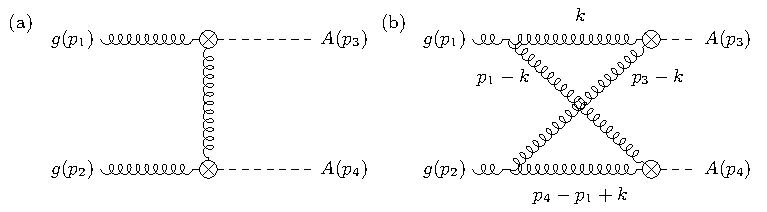
\includegraphics[width=0.95\textwidth]{figures/dps_diagram.pdf}
\caption{DPS configuration in two-loop gluon-fusion amplitudes:
(a) gluon splittings, $gg\to HH$ with effective vertices (crossed circles;
$A$ replaces $H$ for $gg\to AA$); (b) quark splittings, $gg\to ZZ$.
At the equal-mass pinch, $k=xp_1$, $\bar k=(1-x)p_1$, $r=(1-x)p_2$ and
$\bar r=xp_2$ are on shell; $k,r$ enter $\mathcal H_1$ and $\bar k,\bar r$
enter $\mathcal H_2$. Without the additional gluon $\ell$ (red, one
attachment), each panel is the one-loop diagram.}
\label{fig:dps}
\end{figure*}

\textit{Two-loop DPS structure:} Let $\bb$ be the transverse position conjugate to $\boldsymbol p_T$,
$b=|\bb|$. For a given helicity projection and at fixed momentum fractions, the DPS term of the
IR-subtracted amplitude, the part not analytic in $\boldsymbol p_T$ at $\boldsymbol p_T=0$,
is represented as
\begin{equation}
\widetilde{\mathcal A}_{\rm DPS}(b)=\mathcal H_1\mathcal H_2\,\Kt(b),
\label{eq:factorised}
\end{equation}
with $\mathcal H_{1,2}$ the IR-subtracted amplitudes of the two $2\to1$ subprocesses, of
masses $m_1$ and $m_2$, and $\Kt$ a kernel that starts at order $a_s=\alpha_s/(4\pi)$ with one
splitting of each incoming parton. The product denotes contraction over the daughter parton
colour and helicity indices. At one loop this is the factorisation of
Ref.~\cite{Gaunt:2011xd}. At two loops we expand about
the DPS pinch, retaining the leading power in
$\lambda=p_T/\sqrt{s}$ at fixed momentum fractions
away from the endpoints. Hard corrections confined
to either fusion subprocess enter $\mathcal H_i$.
The factorised description assumes the cancellation
of leading hard exchanges between the subprocesses
and the eikonal reduction of soft attachments.
We calculate the collinear, soft, Glauber and ultrasoft
contributions to the kernel and test the resulting
description against complete two-loop amplitudes
in both splitting channels.

The one-loop anomalous dimensions of IR-subtracted amplitudes are determined by the
external partons~\cite{Becher:2009cu}; subtracting those of $\mathcal H_1$ and $\mathcal H_2$ from
that of the $2\to2$ amplitude gives $d\Kt/d\ln\mu=\gamma_{\mathcal K}\Kt$ with
\begin{equation}
\gamma_{\mathcal K}=a_s\Big[-4\DD\ln\frac{Q_*^2}{\mu^2}+4i\pi\DD+2\DG\Big],
\label{eq:gammaK}
\end{equation}
$\DD=C_{R_1}+C_{R_2}-C_a$ and $\DG=\gamma_a-\gamma_{R_1}-\gamma_{R_2}$, where $C_a$ is the Casimir
of the incoming partons, $C_{R_i}$ that of the two partons entering subprocess $i$,
$\gamma_g=-\beta_0$ and $\gamma_q=-3C_F$ are the one-loop non-cusp anomalous dimensions,
$\beta_0=\frac{11}3C_A-\frac43T_Fn_f$.
Colour conservation at the singlet hard vertices gives
$2T_k\cdot T_{\bar r}=\DD$ for exchanges between the
hard vertices, relating this colour factor to
crossed Wilson lines~\cite{Korchemskaya:1994qp}.
The scale $Q_*$ is fixed by
the two outgoing masses and the incoming energy:
$\DD\ln Q_*^2=C_{R_1}\ln m_1^2+C_{R_2}\ln m_2^2-C_a\ln s$.
This combines the mass and energy logarithms
with the corresponding colour factors.
Solving the renormalisation group equation with the
anomalous dimension in Eq.~(\ref{eq:gammaK}) from
$\mu_b=b_0/b$ to $\mu$, where $b_0=2e^{-\gamma_E}$,
and evaluating the coupling of the lowest-order kernel
at $\mu_b$, gives
\begin{equation}
\Kt=a_s\Kt_0\big\{1+a_s\big[\DD X_\mu^2-2\DD XX_\mu+BX_\mu\big]\big\}+a_s^2\widetilde R,
\label{eq:kernel}
\end{equation}
Here $X=\ln(Q_*^2e^{-i\pi}b^2/b_0^2)$,
$X_\mu=\ln(\mu^2b^2/b_0^2)$ and $B=\beta_0+\DG$,
up to $O(a_s^3)$. The renormalisation group determines the scale
dependence of the kernel, while the $\mu$-independent remainder
$\widetilde R$ contains matching information at $\mu_b$.
%We parametrise its two-loop boundary as $\widetilde R=\Kt_0(r_0+r_1X+r_2X^2)$. Here $r_0$ is the finite matching coefficient, while possible terms proportional to $r_1X$ and $r_2X^2$ would change the two-loop logarithms.
We parametrise its two-loop boundary as \(\widetilde R=\widetilde{\mathcal K}_0(r_0+r_1X+r_2X^2)\), where \(r_0\) is the finite matching coefficient and \(r_1,r_2\) represent additional logarithms not fixed by renormalisation group evolution.
%At $\mu^2=Q_*^2e^{-i\pi}$, the bracket in Eq.~(\ref{eq:kernel}) reduces to $-\DD X^2+BX$.
At $\mu^2=Q_*^2e^{-i\pi}$, the RG terms
in Eq.~(\ref{eq:kernel}) reduce to
$-\Delta_C X^2+BX$.

The lowest-order kernel is proportional to $e^{i\nu\phi_b}/b^2$.
We denote the $\nu=0$ and $|\nu|=2$ projections by $\M_1$ and $\M_2$;
for scalar and pseudoscalar pairs these are the equal- and opposite-helicity
amplitudes. For spin-one pairs, $\nu=\Delta J_z$ also includes the outgoing
helicities~\cite{SM}. In momentum space, we define \(\mathcal G=\ln(p_T/Q_*)+i\pi/2\). At one loop, the DPS terms are \(C_1\mathcal G\) in \(\mathcal M_1\) and \(K\) in \(\mathcal M_2\). The difference arises from the Fourier transforms: the isotropic (\(\nu=0\)) integral is logarithmically divergent at small \(b\), whereas the \(|\nu|=2\) integral converges (\hyperref[sec:endmatter]{End Matter}).
%The region calculations and amplitude comparisons below support $r_1=r_2=0$.
The region analysis supports $r_1=r_2=0$ for the DPS
contributions studied. Independent two-loop amplitude fits
find both coefficients consistent with zero within numerical
uncertainties estimated from fit-window variations~\cite{SM}.
With this boundary condition, the terms $-\DD X^2+BX$ give the two-loop logarithms
\begin{equation}
\begin{aligned}
\M_1^{(2)}&\supset C_1\Big[-\tfrac43\DD\,\G^3-B\,\G^2\Big],\\
\M_2^{(2)}&\supset K\Big[-4\DD\,\G^2+(4\DD-2B)\,\G\Big].
\end{aligned}
\label{eq:rg}
\end{equation}
%
For $g\to gg$, $\DD=C_A$ and $B=2\beta_0$.
The two contributions to $B$ arise from the running
coupling of the lowest-order kernel and the non-cusp
anomalous dimensions. The four coefficients in
Eq.~(\ref{eq:rg}) are $-\frac43C_A$, $-2\beta_0$,
$-4C_A$ and $4C_A-4\beta_0$, respectively, with
$Q_*^2=m^4/s$ for equal masses.
For $g\to q\bar q$, $\DD=2C_F-C_A=-1/N_c$ and
$B=6C_F$. The cubic coefficient in $\M_1^{(2)}/C_1$
is $\frac4{3N_c}$, compared with $-\frac43C_A$
for $g\to gg$, reflecting the colour factors in
$\DD$; $\beta_0$ does not enter the quadratic
coefficient, and
$Q_*^2=s^{N_c^2}/m^{2(N_c^2-1)}$.
For $g\to q\bar q$, the Fourier transform is
performed order by order in $a_s$, since the
unexpanded large-$b$ exponent does not yield
a convergent real-$b$ Fourier integral.


The one-loop coefficients follow from the residues of the pinch~\cite{Gaunt:2011xd}.
For two effective vertices and equal final-state masses $m$, the daughter partons
carry longitudinal momentum fractions $x$ and $1-x$ at the DPS pinch,
with $x(1-x)=m^2/s$ [Fig.~\ref{fig:dps}(a)],
\begin{equation}
\begin{aligned}
C_1&=-4\pi iN_c\,x(1-x)\,F_0(x)\,\M_1^{(0)},\\
|K|&=2\pi N_c\,x(1-x)\,F_2(x)\,|\M_1^{(0)}|,
\end{aligned}
\label{eq:oneloop}
\end{equation}
with $\M_1^{(0)}$ the tree-level value of $\M_1$,
$F_0=\frac1{x(1-x)}+2x(1-x)$ for $gg\to HH$,
$F_0\to F_A=\frac1{x(1-x)}-2x(1-x)$ for $gg\to AA$ and $F_2=\frac{x^4+(1-x)^4}{x(1-x)}$ for both processes. These functions arise from the helicity overlaps of the
two splittings~\cite{SM}.
The second relation gives the magnitude of $K$.
In the helicity conventions of the Supplemental Material,
$K>0$ for both $gg\to HH$ and $gg\to AA$.
For $gg\to ZZ$ through a massless quark loop,
$C_1$ is proportional to $x^2$ or $(1-x)^2$,
while $K$ is proportional to $x(1-x)$, depending
on the helicities~\cite{Gaunt:2011xd,SM}.


\textit{Boundary term and phase:}
The potential $X^2$ contribution (Eq.~(\ref{eq:kernel})) comes from ultrasoft exchange. An ultrasoft gluon cannot resolve the transverse separation of the
two hard vertices and couples to the combined colour charge of each
splitting.
%The regulated sum must therefore include attachments to both daughters and their parent. In the static limit, the exchange between the parents cancels the corresponding exchange between the daughters when the same rapidity regulator is used throughout.
The calculation must therefore include diagrams in which the ultrasoft gluon couples to both the daughter partons and their parent gluon.
With the same rapidity regulator throughout, the daughter-daughter and parent-parent exchanges cancel in the static limit, while the mixed parent-daughter contributions vanish.
The calculated soft subtraction also has no finite rapidity logarithm
at $\mu_b=b_0/b$. Together with the two-loop amplitude comparisons,
these results support $r_1=r_2=0$ for the DPS contributions studied.
The remaining finite matching function $r_0$ is determined below.
The Supplemental Material~\cite{SM} gives the regulator and overlap
calculations.

For the leading DPS contribution in Eq.~(\ref{eq:factorised}),
Glauber exchange between partons from the two incoming
splittings generates a phase. Its coefficient is determined
by the colour factor $\DD$, independently of the hard
subprocess amplitudes. With the rapidity regulator and
IR subtraction used here, the poles of the parton
propagators produce an imaginary contribution to the
rapidity logarithm. At fixed momentum
fractions, the dependence of the regions at scale $\mu_b$
on the hard scales enters through $X$ in
Eq.~(\ref{eq:kernel}), with $\operatorname{Im}X=-\pi$.
The imaginary part of the bare kernel is therefore
\begin{equation}
i\,{\rm Im}\,\frac{\Kt^{(1)}_{\rm bare}}{\Kt_0}
=2\pi i\DD\Big[\frac1\epsilon+X_\mu\Big]+O(\epsilon),
\label{eq:imK}
\end{equation}
The $1/\epsilon$ pole is accounted for by the IR subtraction
of the full amplitude relative to the two hard
subprocesses~\cite{Catani:1998bh}. After subtraction, the
phase is given by the $2\pi i\DD X_\mu$ term in
Eq.~(\ref{eq:kernel}). The calculated regions leave no
additional imaginary matching constant at $\mu=\mu_b$.

\textit{Two-loop QCD amplitudes:}
We study the two-loop finite remainders for $gg\to HH$
with effective gluon vertices~\cite{Banerjee:2018lfq},
$gg\to AA$~\cite{Bhattacharya:2019oun},
and $gg\to ZZ$ through massless quark loops~\cite{vonManteuffel:2015msa}.
At fixed velocity $\beta=\sqrt{1-4m^2/s}$,
with $x=(1+\beta)/2$, we approach $p_T=0$
and evaluate the amplitudes using multiprecision
arithmetic. We extract the logarithmic coefficients
by fitting polynomials in $\G$ with $p_T^2$
corrections~\cite{SM}; for $gg\to HH$, omitting
these corrections increases the deviations
to approximately $\plainDevMax$.

For $gg\to HH$ and $gg\to AA$, the coefficients of
$\G^3$ and $\G^2$ in the equal-helicity amplitude,
and of $\G^2$ and $\G$ in the opposite-helicity
amplitude, agree with Eq.~(\ref{eq:rg}) for each of
the colour structures $N_c^2$, $N_cn_f$, $n_f/N_c$
and $n_f^2$.
The comparison covers $\beta=\frac14,\frac12,\frac23$,
with the renormalisation scale dependence of
$gg\to HH$ checked separately.
For $gg\to ZZ$, the predicted logarithms agree
with the two-loop amplitudes in eight helicity
configurations, including symmetry-related ones,
separately for the $C_F$ and
$C_A$ contributions. The fits also confirm the additional
$\ln[x(1-x)]$ terms arising from the different
scale $Q_*$ for quark splittings.
%
We further test Eq.~(\ref{eq:rg}) using the
massless quark $gg\to V_1^*V_2^*$ amplitudes
with different invariant masses for the two
off-shell vector bosons. Up to electroweak couplings,
these amplitudes describe $\gamma^*\gamma^*$, $Z\gamma^*$,
$ZZ$ and $W^+W^-$ pairs~\cite{vonManteuffel:2015msa}.
For $(m_1^2,m_2^2,s)=(1,2,15/2)$
and $(2,3,17)$, in common mass-squared units,
the $++++$ and $++--$ transverse-helicity
amplitudes reproduce the predicted cubic and
quadratic logarithms separately in the $C_F$
and $C_A$ terms. The fits include power
corrections and window variations, as detailed
in the Supplemental Material~\cite{SM}.
%
Figure~\ref{fig:threeprocess} compares the leading and next-to-leading
logarithms across $gg\to HH$, $gg\to AA$ and $gg\to ZZ$.
The normalised cubic coefficients have opposite signs for gluon and
quark splittings. The quadratic coefficient is common to $HH$ and $AA$,
while the $ZZ$ result depends on the splitting momentum fraction
through the scale $Q_*$. The extracted coefficients agree with both
predictions. Table~\ref{tab:tests} gives the corresponding numerical
deviations, fit-window tests and additional velocities.
Together, they support the absence of additional two-loop
boundary logarithms in both splitting channels.
%
\begin{table}[!htb]
\centering
\small
\setlength{\tabcolsep}{3pt}
\begin{tabular}{lccc}
\toprule
& $gg\to HH$ & $gg\to AA$ & $gg\to ZZ$\\
\midrule
Logarithms, Eq.~(\ref{eq:rg}) & $\devLeadMax$ & $\rzAAlead$ & $\zzDevMax$\\
Fit-window shift & $\shiftMax$ & $\rzAALogShift$ & $\zzShiftMax$\\
$r_0$, fitted points & $\rzFitHH$ & $\rzFitAA$ & $\rzFitZZ$\\
$r_0$, extra velocities & $\rzBlindHH$ & $\rzBlindAA$ & $\rzBlindZZ$\\
$r_0$, region numerics & $\rzRegG$ & --- & $\rzRegQ$\\
\bottomrule
\end{tabular}
\caption{Tests of Eqs.~(\ref{eq:rg}), (\ref{eq:r0g})
and~(\ref{eq:r0q}).
The first row gives the largest deviations of the fitted
logarithmic coefficients from Eq.~(\ref{eq:rg}) at
$\beta=\scanBetas$, relative to the nonzero predictions
for $gg\to HH$ and $gg\to AA$, and in units of $C_1$
or $K$ for $gg\to ZZ$.
The second row gives the largest changes upon shifting
the fit window, with the same normalisations as the first row.
The remaining rows give the absolute deviations of $r_0$
from Eqs.~(\ref{eq:r0g}) and~(\ref{eq:r0q}) at the
fitted velocities, at additional velocities
$\beta=\aaBlindBetas$ for $gg\to HH,AA$ and
$\beta=\frac45$ for $gg\to ZZ$, and from numerical integration of the same
region contributions, respectively.
For $gg\to AA$, the modifications described in the
text are applied.}
\label{tab:tests}
\end{table}





\begin{figure*}[!htb]
\centering
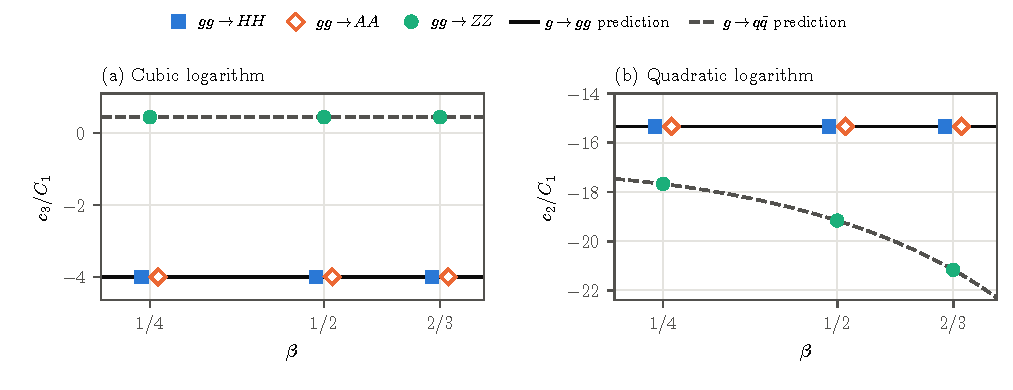
\includegraphics[width=0.94\textwidth]{figures/three_process_comparison.pdf}
\caption{Coefficients of the cubic and quadratic DPS logarithms in the
two-loop $gg\to HH$, $gg\to AA$ and $gg\to ZZ$ amplitudes with
$N_c=3$, $n_f=5$ and
$\mathcal M_1^{(2)}\supset c_3\mathcal G^3+c_2\mathcal G^2$.
Lines are the predictions of Eq.~(\ref{eq:rg}); symbols are coefficients
extracted from the complete amplitudes, divided by the corresponding
one-loop coefficient $C_1$. The $ZZ$ quadratic coefficient is plotted
in the gluon-scale logarithm, as in the amplitude fits; $HH$ and $AA$
share the same prediction. The $HH$ and $AA$ markers are displaced
slightly in $\beta$ to show both sets.}
\label{fig:threeprocess}
\end{figure*}

\textit{Finite matching and parity:}
The finite matching coefficient $r_0$ enters
the term proportional to $\mathcal G$ in
$\M_1^{(2)}$ and the constant term in
$\M_2^{(2)}$. High-precision fits to complete
two-loop amplitudes first identified the constants in $r_0$.
We subsequently derived the matching functions
analytically from the collinear and soft contributions
and parton self-energy corrections~\cite{SM}.
After conversion to a common IR subtraction scheme,
the complete amplitude comparisons confirm the
predicted colour and helicity dependence.
The imaginary part of the extracted $r_0$ is below
$\glauberImag$ in all \glauberValues{} fitted components,
testing the predicted phase in Eq.~(\ref{eq:gammaK}).
We obtain
\begin{align}
r_0^{g\to gg}&=C_A\Big[\tfrac{134}9-5\zeta_2-4\ln x\ln(1-x)\Big]-\tfrac{40}9T_Fn_f\notag\\
&\quad+\frac{2(C_A-2T_Fn_f)}{3F_\nu(x)},\label{eq:r0g}\\
r_0^{g\to q\bar q}&=C_F\Big[12-6\zeta_2+2\ln^2\tfrac{x}{1-x}\Big]\notag\\
&\quad+C_A\Big[2+\zeta_2-2\ln^2x-2\ln^2(1-x)\Big],\label{eq:r0q}
\end{align}
with $x$ the momentum fraction of the splitting and $F_\nu$
the overlap of the component, $F_0$ or $F_2$.
The collinear integrals determine the common finite terms,
while the one-loop splitting tensors and their contraction
with the hard amplitudes determine the helicity dependence.
The last term of Eq.~(\ref{eq:r0g}) carries this dependence,
whereas $r_0^{g\to q\bar q}$ is helicity independent.
For $gg\to AA$, $F_A$ replaces $F_0$ for $\nu=0$,
while the last term changes sign for $\nu=2$.

The amplitude reconstruction uses three velocities
and is tested at additional velocities
(Table~\ref{tab:tests}).
The collinear and soft rapidity poles cancel analytically
for $0<x<1$. Numerical integration of the same
region contributions at $x=0.1$, $0.3$ and $0.5$
confirms the matching functions in the tested colour
and helicity channels.
At $x=1/2$ and $\mu_R=m_A$, the $gg\to AA$ prediction
from Eq.~(\ref{eq:r0g}) reproduces the coefficient of
$\G$ in Eq.~(4.6) of Ref.~\cite{P1} exactly, including
the hard contribution and finite IR-scheme conversion.
The helicity-dependent term of Eq.~(\ref{eq:r0g}) originates from the
rational part of the one-loop $g\to gg$ splitting amplitudes~\cite{Bern:1999ry}, with colour factor $C_A-2T_Fn_f$.
For $\nu=2$, the helicity-flip contribution has the relative sign
of $M_{--}/M_{++}$ of the hard vertex.

\textit{Planar $\mathcal N=4$ checks:}
The known self-crossing limit of six-gluon
amplitudes, related to the evolution of
intersecting Wilson lines~\cite{Korchemskaya:1994qp,Dixon:2016epj},
provides a separate setting in which to test
the angular decomposition~\cite{CaronHuot:2019vjl}.
We use the BDS-like normalisation of the six-gluon amplitude,
which divides out a modified Bern-Dixon-Smirnov (BDS)
factor~\cite{Dixon:2016epj}. For $a=g^2N_c/(8\pi^2)$,
the Sudakov factor of Ref.~\cite{Dixon:2016epj} is
\begin{equation}
\begin{aligned}
\mathcal S(a,X)
&=\exp\left[-\frac{\gamma_K(a)}8X^2+B(a)X\right],\\
\gamma_K(a)
&=4a-4\zeta_2a^2+22\zeta_4a^3
+\gamma_K^{(4)}a^4+\ldots .
\end{aligned}
\label{eq:n4exp}
\end{equation}
%
Here $\gamma_K$ is the cusp anomalous dimension~\cite{Beisert:2006ez}, distinct from the kernel
anomalous dimension $\gamma_{\mathcal K}$ in
Eq.~(\ref{eq:gammaK}), and
$B(a)=\sum_{n\ge2}B^{(n)}a^n$.
The prefactor $a\Kt_0(1+\sum_n\kappa_na^n)$
multiplies $\mathcal S(a,X)$ and includes the
hard functions and BDS-like normalisation.
In $3\to3$ kinematics, the phase cancels and
$\G=\tfrac12\ln|\delta_*|$, with
$\delta_*=p_T^2/Q_*^2$.
The MHV singularity corresponds to $\nu=0$,
with $C_1=2\pi i$.
With the normalisation and boundary constants
fixed, the representation reproduces \nFourPass{}
additional logarithmic coefficients of the known
planar six-gluon amplitudes through five loops
(Table~\ref{tab:n4letter},
\hyperref[sec:endmatter]{End Matter}).


In the $v\to0^-$ overlap with multi-Regge kinematics, the selected
next-to-MHV component carries $|\Delta J_z|=2$. The transform with
$\nu=2$ reproduces \nFourNmhvChecked{} coefficients through four loops
and \nFourNmhvFiveCount{} five-loop coefficients obtained from the
published multi-Regge amplitude~\cite{CaronHuot:2019vjl}, without an
additional matching constant. For the leading nonanalytic terms,
$\M_2(\G)/K=\int_0^\infty ds\,e^{-s}C_1^{-1}
\partial_\G\M_1(\G-s/2)$ follows from the known helicity-flip
factor~\cite{Basso:2014bfkl,CaronHuot:2019vjl}. These are consistency
tests of the DPS interpretation, not a new all-order relation.


The region calculation in planar $\mathcal N=4$ theory,
combined with the hard amplitudes and BDS-like
normalisation, yields $\kappa_1=\zeta_2$, with
deviations below \kappaOneReg{} for \nFourRegPairs{}
pairs of splitting fractions in the four-dimensional
helicity scheme. The $\mathcal N=4$ field content
cancels the rational helicity-dependent term, giving
identical finite matching coefficients for the two
angular components. The Supplemental Material details
the normalisation and analytic continuation to $2\to4$
kinematics, including the phase in
Eq.~(\ref{eq:imK}).



\textit{Three loops:}
The kernel evolution also yields conditional predictions
for the leading three-loop DPS logarithms. If the
factorised description persists and the boundary
correction at relative order $a_s^2$ contains no
powers of $X$ higher than $X^2$, the two highest
logarithmic powers in each component are fixed.
The third is fixed if the $X^2$ coefficient also
vanishes. These boundary conditions remain to be
tested at three loops~\cite{SM}.

Under both conditions, the relative boundary correction
is $a_sr_0+a_s^2(r_0^{(3)}+r_1^{(3)}X)$, with $a_s$
evaluated at $\mu_b$.
The leading three-loop logarithms follow from the
renormalisation group evolution with the known
two-loop cusp anomalous dimension
$\gamma_{\rm cusp}(a_s)=4a_s+\Gamma_1a_s^2$,
where
$\Gamma_1=4[(67/9-2\zeta_2)C_A-20T_Fn_f/9]$.
Using the running coupling and the boundary
conditions stated above, we obtain in
minimal subtraction
\begin{equation}
\begin{aligned}
\M_1^{(3)}&\supset C_1\Big[\tfrac85\DD^2\G^5+c_4\G^4+c_3^{(0)}\G^3\Big],\\
\M_2^{(3)}&\supset K\Big[8\DD^2\G^4+(4c_4-16\DD^2)\G^3\\
&\qquad+\big(3c_3^{(2)}-4\DD(3B+2\beta_0-6\DD)\big)\G^2\Big].
\end{aligned}
\label{eq:threeloop}
\end{equation}
Here
$c_4=2\DD(B+\frac23\beta_0)$ and
$c_3^{(\nu)}=\frac23B(B+\beta_0)-\frac13\DD\Gamma_1-\frac83\DD h-\frac43\DD r_0^{(\nu)}-\frac43\DD L_*(B+\beta_0+\DD L_*)$.
Here $r_0^{(\nu)}$ is the finite matching coefficient
of the corresponding component, $h$ is the one-loop
hard correction relative to the tree amplitude
for either of the identical subprocesses, and
$L_*=\ln[\mu^2/(Q_*^2e^{-i\pi})]$.

For gluon splittings with $T_F=\frac12$, the
coefficients of the two highest powers are
$\frac85C_A^2$ and
$\frac{176}9C_A^2-\frac{32}9C_An_f$
in $\M_1^{(3)}/C_1$, and $8C_A^2$ and
$\frac{560}9C_A^2-\frac{128}9C_An_f$
in $\M_2^{(3)}/K$.
These coefficients are independent of the
renormalisation scale and IR subtraction
scheme. Table~\ref{tab:threeloop}
(\hyperref[sec:endmatter]{End Matter})
gives the third coefficient for $gg\to HH$.


\textit{Conclusion:}
We have determined the DPS singularity of gluon-fusion
amplitudes at two loops, including its finite matching
functions, for gluon and quark splittings.
A single colour factor, $\DD$, controls both the cubic
logarithm and the phase generated by Glauber exchange;
it is positive for gluon splittings and negative for
quark splittings. The helicity and parity dependence
of the finite matching functions follows from the
one-loop splitting tensors.
Because the final state enters only through the hard
subprocess amplitudes and one hard scale, the kernel
determines the leading two-loop logarithms for massive
colour-singlet pair production with the DPS configuration
studied here, without an expansion of the two-loop amplitude.
The predictions agree with complete two-loop amplitudes
in both splitting channels, with amplitudes for off-shell
vector bosons of unequal invariant masses and with known
planar $\mathcal N=4$ results through five loops.
They provide analytic benchmarks for complete two-loop
calculations and, under the stated boundary conditions,
extend to the leading three-loop logarithms.

\begin{acknowledgments}
I thank IFIC, University of Valencia, and Prof. Francisco Campanario for providing the computing resources used in this work.
ChatGPT (OpenAI) and Claude (Anthropic) were used to
draft notes, draft and debug code, and organise the Git
repository.
%Their use in the computational work and the verification procedures are described in the Supplemental Material~\cite{SM}.
The author takes full responsibility for the content of this Letter.
\end{acknowledgments}

\textit{Data availability:} The scripts, stored amplitude points, numerical
results and validation tests accompanying this work are supplied in the
\texttt{anc/} directory of the arXiv source archive and in the companion
repository at \url{https://github.com/abhattacharya1992/two-loop-dps-prl}.
The additional $gg\to V_1^*V_2^*$ scan records and precision checks are in \texttt{paper2/unequal\_virtuality/} of the companion repository.
Re-evaluation from the original published two-loop amplitudes requires
the external inputs identified in the repository README.

% generated by make_tables.py; needed for clean arXiv compilation
\nocite{Ahmed:2015qpa,Bauer:2001yt,Bauer:2002nz,Becher:2009qa,Bern:1994zx,Bern:2005iz,Binoth:2000ps,Buffing:2017mqm,Caola:2015ila,Catani:2011spacelike,Catani:2013tia,Coleman:1965xm,Diehl:2019rdh,Dixon:1996wi,Dixon:2012yy,Echevarria:2011epo,Eden:1966dnq,Forshaw:2012breaking,Frellesvig:2016ske,Gardi:2009qi,Gardi:2024dissecting,Gehrmann:2015ora,Henn:2014lfa,Kosower:1999xi,Landau:1959fi,Mangano:1990by,Passarino:1978jh,Rothstein:2016glauber,mpmath}

\bibliography{references,sm}

\section*{End Matter}\phantomsection\label{sec:endmatter}

% The planar N = 4 table is input before its text: as a two-column float it can only go to the top of a
% page, so defined here, on the page where the references end, it lands at the top of the next one.
\begin{table*}[!htb]
\centering
\small
\setlength{\tabcolsep}{5pt}
\begin{tabular}{@{}r@{\hspace{4pt}}r@{\hspace{6pt}}l@{\hspace{12pt}}r@{\hspace{4pt}}r@{\hspace{6pt}}l@{}}
\toprule
\multicolumn{3}{c}{\textbf{MHV}: $2\pi i\,\ell^k$} & \multicolumn{3}{c}{\textbf{NMHV}: $\pi i\,\frac{1+w}{1+w^*}\,\ell^k$}\\
\cmidrule(lr){1-3}\cmidrule(l){4-6}
$L$ & $k$ & coefficient & $L$ & $k$ & coefficient\\
\midrule
1 & 1 & $\tfrac{1}{2}$ & 1 & 0 & $1$\\
\addlinespace[3pt]
2 & 3 & $- \tfrac{1}{12}$ & 2 & 2 & $- \tfrac{1}{2}$\\
 & 2 & $0$ &  & 1 & $1$\\
 & 1 & $\tfrac{\zeta_{2}}{2}\,[\kappa_1]$ &  & 0 & $\zeta_{2} - 1$\\
\addlinespace[3pt]
3 & 5 & $\tfrac{1}{80}$ & 3 & 4 & $\tfrac{1}{8}$\\
 & 4 & $0$ &  & 3 & $- \tfrac{1}{2}$\\
 & 3 & $0$ &  & 2 & $\tfrac{3}{2}$\\
 & 2 & $- \tfrac{\zeta_{3}}{4}\,[B^{(2)}]$ &  & 1 & $- \zeta_{3} - 3$\\
 & 1 & $\tfrac{\zeta_{4}}{4}\,[\kappa_2]$ &  & 0 & $\zeta_{3} + \tfrac{\zeta_{4}}{2} + 3$\\
\addlinespace[3pt]
4 & 7 & $- \tfrac{1}{672}$ & 4 & 6 & $- \tfrac{1}{48}$\\
 & 6 & $0$ &  & 5 & $\tfrac{1}{8}$\\
 & 5 & $- \tfrac{\zeta_{2}}{80}$ &  & 4 & $- \tfrac{\zeta_{2}}{8} - \tfrac{5}{8}$\\
 & 4 & $- \tfrac{\zeta_{3}}{48}$ &  & 3 & $\tfrac{\zeta_{2}}{2} - \tfrac{\zeta_{3}}{6} + \tfrac{5}{2}$\\
 & 3 & $- \tfrac{7 \zeta_{4}}{24}$ &  & 2 & $- \tfrac{3 \zeta_{2}}{2} + \tfrac{\zeta_{3}}{2} - \tfrac{7 \zeta_{4}}{4} - \tfrac{15}{2}$\\
 & 2 & $- \tfrac{3 \zeta_{2} \zeta_{3}}{4} + \zeta_{5}\,[B^{(3)}]$ &  & 1 & $- 3 \zeta_{2} \zeta_{3} + 3 \zeta_{2} - \zeta_{3} + \tfrac{7 \zeta_{4}}{2} + 4 \zeta_{5} + 15$\\
 & 1 & $- \zeta_{3}^{2} - \tfrac{13 \zeta_{6}}{48}\,[\kappa_3]$ &  & 0 & $3 \zeta_{2} \zeta_{3} - 3 \zeta_{2} - 2 \zeta_{3}^{2} + \zeta_{3} - \tfrac{7 \zeta_{4}}{2} - 4 \zeta_{5} - \tfrac{13 \zeta_{6}}{24} - 15$\\
\midrule
\multicolumn{6}{@{}l}{\textbf{MHV}, $L=5$: $2\pi i\,\ell^k$}\\
\cmidrule(l){1-6}
5 & 9 & $\tfrac{1}{6912}$ & 5 & 4 & $\tfrac{7 \zeta_{2} \zeta_{3}}{24} + \tfrac{\zeta_{5}}{4}$\\
 & 8 & $0$ &  & 3 & $\tfrac{2 \zeta_{3}^{2}}{3} + \tfrac{115 \zeta_{6}}{72}\,[\gamma_K^{(4)}]$\\
 & 7 & $\tfrac{\zeta_{2}}{336}$ &  & 2 & $\tfrac{17 \zeta_{2} \zeta_{5}}{4} + \tfrac{11 \zeta_{3} \zeta_{4}}{4} - \tfrac{55 \zeta_{7}}{16}\,[B^{(4)}]$\\
 & 6 & $\tfrac{5 \zeta_{3}}{288}$ &  & 1 & $\tfrac{\zeta_{2} \zeta_{3}^{2}}{4} + \tfrac{45 \zeta_{3} \zeta_{5}}{4} + \tfrac{257 \zeta_{8}}{72}\,[\kappa_4]$\\
 & 5 & $\tfrac{9 \zeta_{4}}{80}$ & & & \\
\bottomrule
\end{tabular}
\caption{Planar $\mathcal N=4$: the coefficients of the powers of $\ell=\ln|\delta_*|$ in the $L$-loop MHV amplitude $\mathcal E^{(L)}$, Eqs.~(3.17)--(3.21) of Ref.~\cite{Dixon:2016epj}, and in the next-to-MHV amplitude $\rho^{(L)}$, Eqs.~(D.14)--(D.17) of its erratum, in $3\to3$ kinematics, against Eqs.~(\ref{eq:kernel}), (\ref{eq:Fm}) and~(\ref{eq:n4exp}) with $\nu=0$ and $\nu=2$. The one-loop coefficients define $C_1$ and $K$; a coefficient followed by a constant in brackets fixes that constant, and the remaining coefficients check the known radial representation and helicity map. All agree.}
\label{tab:n4letter}
\end{table*}

\textit{Appendix A: Transforms:} The Fourier transforms of the two components of $\Kt_0$ with
$X^n$ inserted follow by differentiating
\begin{equation}
\begin{aligned}
\Phi_\nu(\alpha)&=\int\!\frac{d^2\bb}{2\pi}\frac{e^{i\boldsymbol p_T\cdot\bb+i\nu\phi_b}}{b^2}
\Big(\frac{Q_*^2e^{-i\pi}b^2}{b_0^2}\Big)^{\!\alpha}\\
&=\frac{i^\nu e^{i\nu\phi_q}}{2}\,e^{2(\gamma_E-\G)\alpha}\,
\frac{\Gamma(\frac\nu2+\alpha)}{\Gamma(1+\frac\nu2-\alpha)}
\end{aligned}
\label{eq:Fm}
\end{equation}
at $\alpha=0$, with $\phi_q$ the azimuth of
$\boldsymbol p_T$. For $\nu=0$, the pole of
$\Gamma(\alpha)$ is independent of $p_T$ and
corresponds to a contact term in impact-parameter
space, which is omitted from the nonanalytic
DPS part of the amplitude.
The finite part contains one additional power of $\G$.
No such pole occurs for $\nu=2$.


\begin{table}[!htb]
\centering
\footnotesize
\setlength{\tabcolsep}{7pt}
\begin{tabular}{lccc}
\toprule
$x$ & $N_c^2$ & $N_cn_f$ & $n_f^2$\\
\midrule
\multicolumn{4}{@{}l}{$[\G^3]\,\M_1^{(3)}/C_1$}\\
$\frac58$ & $-0.008-58.231\,i$ & $-11.055+8.378\,i$ & $1.778$\\
$\frac34$ & $-4.510-60.101\,i$ & $-10.491+8.378\,i$ & $1.778$\\
$\frac56$ & $-10.719-62.615\,i$ & $-9.728+8.378\,i$ & $1.778$\\
\midrule
\multicolumn{4}{@{}l}{$[\G^2]\,\M_2^{(3)}/K$}\\
$\frac58$ & $-96.420-174.693\,i$ & $-8.767+25.133\,i$ & $5.333$\\
$\frac34$ & $-107.957-180.302\,i$ & $-9.047+25.133\,i$ & $5.333$\\
$\frac56$ & $-125.901-187.844\,i$ & $-7.441+25.133\,i$ & $5.333$\\
\bottomrule
\end{tabular}
\caption{Conditional three-loop DPS coefficients for $gg\to HH$ at $\mu=m_H$ in minimal subtraction; the boundary assumptions are stated in the text.}
\label{tab:threeloop}
\end{table}



\textit{Appendix B: The boundary term from the regions:}
We apply the method of regions~\cite{Beneke:1997zp}
to the two-loop DPS term at leading power in $\lambda$.
We use dimensional regularisation and a common
rapidity regulator, with scaleless integrals set to
zero in the adopted prescription. Collinear, soft
and Glauber gluons have transverse momenta of order
$p_T$ and resolve the separation $b$. Their transverse
scale is $\mu_b$, while the hard-scale dependence
enters via a regulated rapidity logarithm at
this order~\cite{Chiu:2012ir}.

An ultrasoft gluon has light-cone and transverse
momentum components
$\ell^+\sim\ell^-\sim|\boldsymbol\ell_\perp|
\sim p_T^2/\sqrt{s}$.
Since $|\boldsymbol\ell_\perp|b\ll1$,
it does not resolve the transverse separation $b$.
However, $p_1^+\ell^-$ and $p_2^-\ell^+$
are of order $p_T^2$ and therefore contribute
to the denominators of the nearly on-shell
parton propagators.
Denoting the dimensionful
light-cone energy denominators of the two splittings
by $\sigma_1$ and $\sigma_2$, their product scales as
$\sigma_1\sigma_2\sim\mu_b^4s/(m_1^2m_2^2)$, or
$\mu_b^4/Q_*^2$ for gluon splittings.
An individual exchange between daughter partons
contains a factor
$\Gamma(\epsilon)^2\Gamma(1-\epsilon)
(\sigma_1\sigma_2e^{i\pi}/\mu^2)^{-\epsilon}$,
which can generate an $X^2$ boundary term.

At leading eikonal power, colour conservation
combines the daughter charges into their parent
charge, $T_k+T_{\bar k}=T_{p_1}$, and similarly
for the second splitting. With the same regulator
for all attachments, the static daughter-daughter
contribution $-2\pi^2$ cancels the parent-parent
term $+2\pi^2$; mixed terms vanish~\cite{SM}.
The Glauber phase is treated separately in Appendix C.

After combining the momentum-region contributions
with the required overlap subtractions, their
Laurent expansions have the form
$(\mu^2/\Lambda^2)^\epsilon
(e_2/\epsilon^2+e_1/\epsilon+e_0)$.
For the collinear, soft and Glauber contributions,
$\Lambda=\mu_b$. Their hard-scale dependence enters
through the rapidity logarithm
$(g/\epsilon+g_1)\ln(Q_*^2e^{-i\pi}/\mu_b^2)$;
ultrasoft terms use
$\Lambda^2=\mu_b^4/(\kappa Q_*^2e^{-i\pi})$,
with $\kappa$ independent of $b$.
Independence of the IR poles from $b$, followed
by subtraction, gives $r_2=e_2^{\rm us}/2$ and
$r_1=g_1+e_1^{\rm us}+e_2^{\rm us}\ln\kappa$.
The regulated ultrasoft cancellation gives
$r_2=0$ and $r_1=g_1$ for the calculated terms.

The soft and collinear rapidity poles cancel.
Their sum yields $2\DD$ times the Fourier
transform of $1/\boldsymbol\ell^2$ in
$2-2\epsilon$ dimensions at separation $b$,
\begin{equation}
\Big(\frac{\mu^2b^2}{b_0^2}\Big)^\epsilon e^{-\epsilon\gamma_E}\Gamma(-\epsilon)
=\Big(\frac{\mu^2}{\mu_b^2}\Big)^\epsilon\Big(-\frac1\epsilon-\frac{\zeta_2}2\epsilon+O(\epsilon^2)\Big).
\label{eq:rapcoef}
\end{equation}
At $\mu=\mu_b$ the finite part vanishes,
giving $g_1=r_1=0$. The resulting boundary
coefficients agree with the two-loop amplitudes;
the imaginary term in Eq.~(\ref{eq:imK}) follows
from the same coefficient multiplied by $-i\pi$.




\textit{Appendix C: Glauber exchange:}
In the rapidity-regulator and overlap-subtraction scheme
of Ref.~\cite{Chiu:2012ir}, the phase in
Eq.~(\ref{eq:imK}) arises from the Glauber region.
For an exchange between a daughter parton from each
incoming splitting, the off-shell propagators reduce
at leading power to eikonal denominators with positive
light-cone energy offsets $\sigma_1$ and $\sigma_2$.
Integrating over the longitudinal components of the
exchanged gluon gives
\begin{equation}
\frac{2\pi i}{\boldsymbol\ell^2+\sigma_1\sigma_2}\Big[\ln\frac{\boldsymbol\ell^2}{\sigma_1\sigma_2}-i\pi\Big],
\label{eq:glauberpair}
\end{equation}
where the pole at $\ell^-=\sigma_1$ lies within the
integration range and produces the $-i\pi$ term.
The logarithm is the rapidity logarithm, with
$\sigma_1\sigma_2\sim\mu_b^4/Q_*^2$.

Soft and collinear rapidity poles cancel; the Glauber
region supplies the phase in Eq.~(\ref{eq:glauberpair}).
Zero bins vanish in this prescription, while delta
and principal-value terms contribute equally~\cite{SM}.
The phase cancels for incoming--outgoing pairs
($\sigma_2<0$). Direct longitudinal integration checks
\glauberConfigs{} configurations in a two-loop graph~\cite{SM}.

%\begin{table}[!htb]
\centering
\footnotesize
\setlength{\tabcolsep}{7pt}
\begin{tabular}{lccc}
\toprule
$x$ & $N_c^2$ & $N_cn_f$ & $n_f^2$\\
\midrule
\multicolumn{4}{@{}l}{$[\G^3]\,\M_1^{(3)}/C_1$}\\
$\frac58$ & $-0.008-58.231\,i$ & $-11.055+8.378\,i$ & $1.778$\\
$\frac34$ & $-4.510-60.101\,i$ & $-10.491+8.378\,i$ & $1.778$\\
$\frac56$ & $-10.719-62.615\,i$ & $-9.728+8.378\,i$ & $1.778$\\
\midrule
\multicolumn{4}{@{}l}{$[\G^2]\,\M_2^{(3)}/K$}\\
$\frac58$ & $-96.420-174.693\,i$ & $-8.767+25.133\,i$ & $5.333$\\
$\frac34$ & $-107.957-180.302\,i$ & $-9.047+25.133\,i$ & $5.333$\\
$\frac56$ & $-125.901-187.844\,i$ & $-7.441+25.133\,i$ & $5.333$\\
\bottomrule
\end{tabular}
\caption{Conditional three-loop DPS coefficients for $gg\to HH$ at $\mu=m_H$ in minimal subtraction; the boundary assumptions are stated in the text.}
\label{tab:threeloop}
\end{table}


\end{document}
